\documentclass{article}
\usepackage{geometry}
\usepackage{graphicx}
\usepackage{makeidx}
\usepackage{wrapfig}

\makeindex
\geometry{
a4paper,
top=10mm,
bottom=15mm,
left=10mm,
right=10mm,
}

\begin{document}

\pagenumbering{gobble}

\newgeometry{
top=30mm,
bottom=20mm,
left=20mm,
right=20mm,
}

\begin{center}
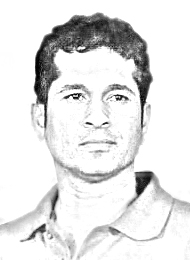
\includegraphics[width=0.3\columnwidth]{Sachin.jpg}\\
\vspace{10pt}
\textbf{\Huge Sachin Tendulkar} \\
\vspace{20pt}
{\large An Article for Assignment 6 on \LaTeX } \\
\textbf{\large CS251: Computer Laboratory} \\
\vspace{30pt}

\textbf{\large Jayant Agrawal} \\
(14282)
\vspace{20pt}

INSTRUCTOR \\
\textbf{Prof. Arnab Bhattacharya}
\vspace{30pt}


\includegraphics[width=0.3\columnwidth]{logo.jpg}\\
\textbf{\large Department of Comuter Science and Engineering \\
INDIAN INSTITUTE OF TECHNOLOGY KANPUR \\
KANPUR 208016, INDIA \\ }
\vspace{10pt}
Feb 2016

\end{center}
\newpage
\pagenumbering{roman}

\begin{center}

\textbf{\Large Sir Donald Bradman\\}
"I see myself when I see Sachin Batting"
\vspace{80pt}

\textbf{\Large Brian Lara}\\
"Tendulkar is to Cricket what Michael Jordan is to Basketball and Muhammad Ali is to Boxing"
\vspace{80pt}

\textbf{\Large Hashim Amla}\\
"Nothing bad can happen to us if we're on a plane in India with Sachin Tendulkar on it"
\vspace{80pt}

\textbf{\Large Time Magazine}\\
"We have had champions, we have had legends, but we have never had another Sachin Tendulkar and we never will"
\vspace{80pt}

\textbf{\Large Matthew Hayden}\\
"I have seen God. He bats for India a number 4 in Tests"
\vspace{80pt}

\textbf{\Large A fan at the SCG}\\
"Commit all your crimes when Sachin is batting. They will go unnoticed for even the Lord is busy watching him"

\vspace{80pt}
\cite{scoop}
\end{center}


\restoregeometry
\newpage
\tableofcontents
\addcontentsline{toc}{section}{\listfigurename}
\addcontentsline{toc}{section}{\listtablename}
\listoffigures
\listoftables

\newpage
\pagenumbering{arabic}
{
\begin{wrapfigure}{R}{0.45\textwidth}
\vspace{-100pt}
\begin{center}
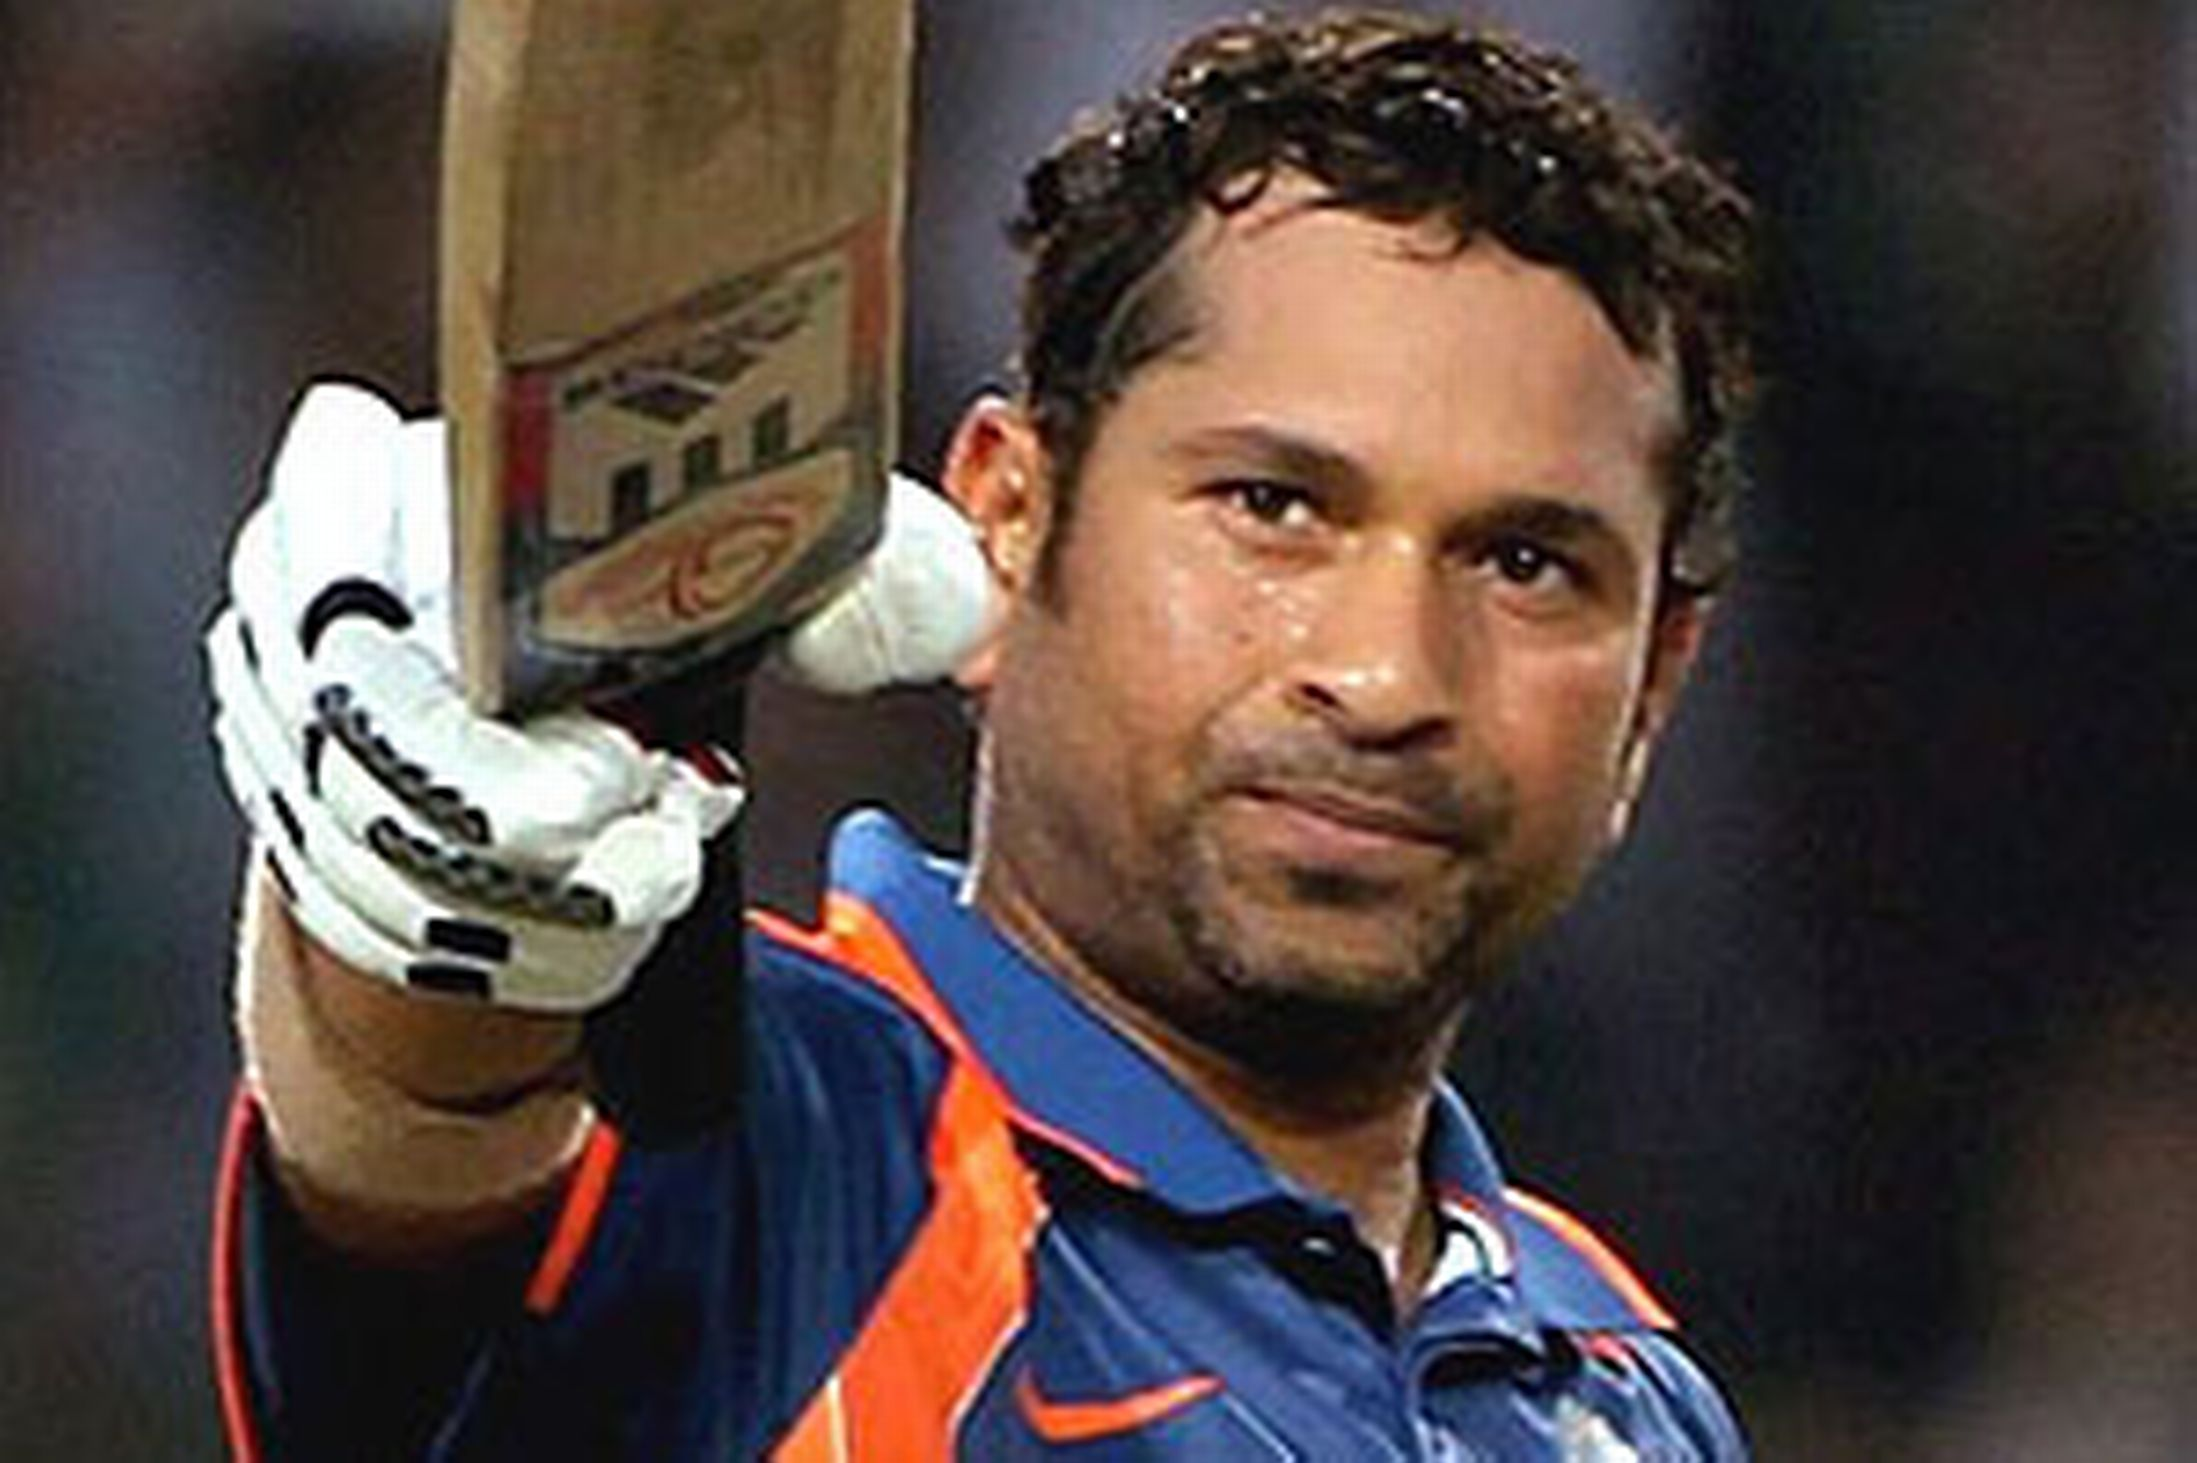
\includegraphics[width=0.3\textwidth]{sachin2.jpg}
\caption{First ever ODI double century}
\end{center}
\end{wrapfigure}
\section{Player Information}
\begin{tabular}{l l}
\textbf{Full Name} & Sachin Ramesh Tendulkar \\
\textbf{Born} & 24 April 1973 \\
\textbf{Height} & 5 ft 5 in (165 cm) \\
\textbf{Batting Style} & Right-handed \\
\textbf{Relations} & \textbf{Wife: } Anjali Tendulkar \\
& \textbf{Daughter: }  Sara Tendulkar \\
& \textbf{Son: } Arjun Tendulkar \\
\textbf{Test Debut} & 15 November 1989 v Pakistan \\
\textbf{Last Test} & 14 November 2013 v West Indies \\
\textbf{ODI debut} & 18 December 1989 v Pakistan \\
\textbf{Last ODI} & 18 March 2012 v Pakistan \\
\textbf{Only T20} & 1 December 2006 v South Africa \\
\end{tabular}
}
\newline \\
Source : \cite{wiki}

\section{Introduction}
\textbf{Sachin Ramesh Tendulkar} is a former Indian cricketer and captain, widely regarded as one of the greatest batsmen of all time. He took cricket \index{cricket} at the age of eleven, made his Test \index{Test} debut \index{debut} on 15 November 1989 against Pakistan in Karachi at the age of sixteen, and went on to represent Mumbai domestically and India internationally for close to twenty-four years. He is the only player to have scored one hundred international \index{centuries} centuries, the first \index{batsmen} batsman to score a double century in a \index{One Day International} One Day International, holds the \index{record} record for most number of \index{runs} runs in both ODI and \index{Test} Test cricket, the only player to complete more than 30,000 runs in international cricket. \cite{wiki} \\

There are so many things that Sachin Tendulkar is to so many people, that it is sometimes forgotten that he is first and foremost a batsman of unparalleled ability, dedication and mind. If he had taken to some other sport in early childhood, his persona would have been invented -- by coaches who want to teach their wards the virtues a tight technique that allows attacking shots, by film-makers who want to create celluloid fantasy by depicting the perfect batsman and superstar, by marketing men who want to appeal to the broadest strata of public imaginable and by cricket fanatics who want to see batting perfection embodied in one person. \cite{cric} \\ 

\section{Captaincy}
Tendulkar's two \index{tenures} as captain of the Indian cricket team were not very successful. When Tendulkar took over as \index{captain} in 1996, it was with huge hopes and expectations. However, by 1997 the \index{team} was performing poorly.
Table \ref{table:cap} shows his captaincy stint.

\begin{table}[h1]
\begin{center}
\begin{tabular}{|c|c|c|c|c|c|c|c|}
\hline
& {\bf Matches} & {\bf Won} & {\bf Lost} & {\bf Drawn} & {\bf Tied} & {\bf NR} & {\bf Win\%} \\
\hline
{\bf Test} & 25 & 4 & 9 & 12 & 0 & - & 16\% \\
{\bf ODI} & 73 & 23 & 43 & - & 2 & 6 & 31\% \\
\hline
\end{tabular}
\caption{Tendulkar's record as captain \cite{wiki}}
\label{table:cap}
\end{center}
\end{table}
	
\section{Playing Style}
Sachin's batting is based on complete balance and poise while limiting unnecessary \index{movements} movements and flourishes. He appears to show little preference for the slow and low wickets which are typical in India, and has scored many centuries on the hard, bouncy pitches in South Africa and Australia.He is known for his unique \index{punch} punch style of hitting the ball over \index{square} square. He is also renowned for his picture-perfect \index{straight} straight \index{drive} drive, often completed with no follow-through. The straight drive is often said to be his favourite shot.
Figure 2 shows how he favours the covers and mid-wicket region the most. \\
\newpage
\begin{figure}[h!]
\begin{center}
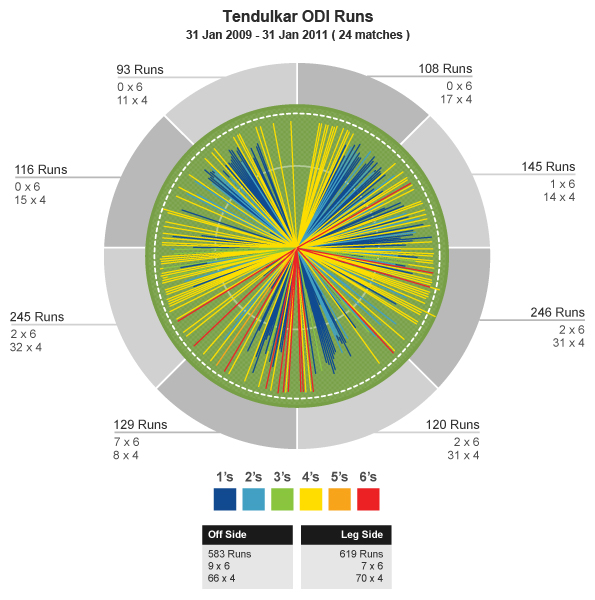
\includegraphics[width=0.5\textwidth]{chart.jpg}
\label{fig:chart}
\caption{Wagon-wheel from year 2009-11} 
\end{center}
\end{figure}


\section{Batting Career Summary}
\begin{table}[h!]
\begin{center}
\begin{tabular}{l r r r r r r r r r r r}
\hline
& {\bf M} & {\bf Inn} & {\bf Runs} & {\bf HS} & {\bf Avg} & {\bf SR} & {\bf 100} & {\bf 200} & {\bf 50} & {\bf 4s} & {\bf 6s} \\
\hline
{\bf Tests} & 200 & 329 & 15921 & 248 & 53.79 & 54.08 & 51 & 6 & 68 & 2058 & 69 \\
{\bf ODI} & 463 & 452 &18426&200 & 44.83 & 86.24 & 49 & 1 & 96 & 2016 & 195 \\
{\bf T20} & 1 & 1 & 10 & 10 & 10 & 83.33 & 0 &0 & 0 & 2 & 0 \\
{\bf IPL} & 78 & 78 & 2334 & 100 & 33.83 & 119.82 & 1 & 0 & 13 & 295 & 29 \\
\hline
\end{tabular}
\caption{Bating Career Summary \cite{cric} }
\end{center}
\end{table}

\section{Career breakdown}
\begin{figure}[h!]
\begin{center}
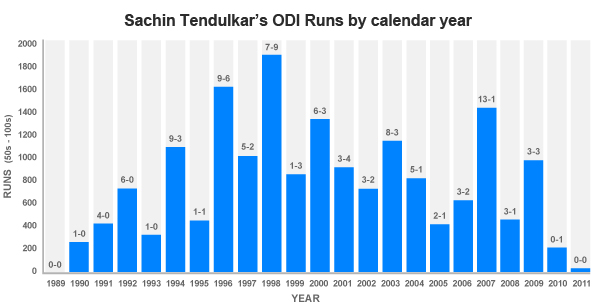
\includegraphics[width=0.5\textwidth]{odi.jpg}
\label{fig:odi}
\caption{ODI batting performance (yearly) }
\end{center}
\end{figure}


\begin{figure}[h!]
\begin{center}
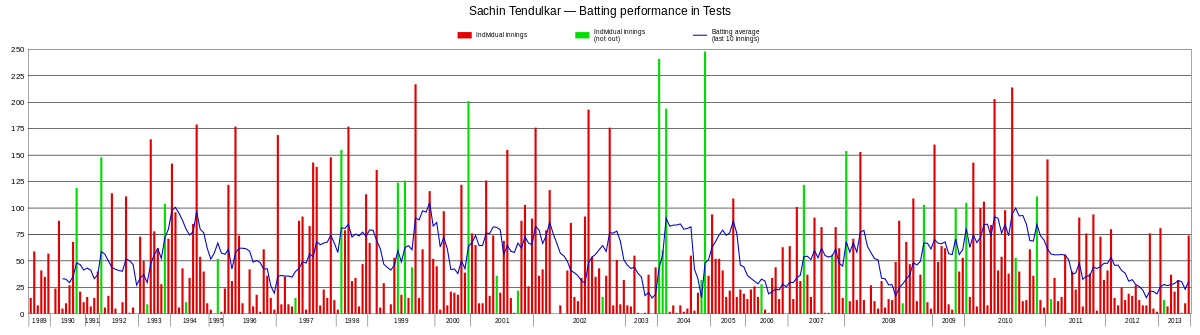
\includegraphics[width=0.9\textwidth]{test.png}
\label{fig:test}
\caption{Test batting performance(per inning)} 
\end{center}
\end{figure}



\section{Achievements and Awards}
\subsection{National Honours \cite{wiki}}
\begin{itemize}
\item 1994 – Arjuna Award, by the Government of India in recognition of his outstanding achievement in sports.
\item 1997-98 – Rajiv Gandhi Khel Ratna, India's highest honour given for achievement in sports.
\item 1999 – Padma Shri, India's fourth highest civilian award.
\item 2001 – Maharashtra Bhushan Award, Maharashtra State's highest Civilian Award.
\item 2008 – Padma Vibhushan, India's second highest civilian award.
\item 2014 - Bharat Ratna, India's highest civilian award.
\end{itemize}

\subsection{Other Honours \cite{wiki}}
\begin{itemize}
\item 2003 – Player of the tournament in 2003 Cricket World Cup.
\item 2004, 2007, 2010 – ICC World ODI XI.
\item 2009, 2010, 2011 – ICC World Test XI.
\item 2010 – Outstanding Achievement in Sport and the Peoples Choice Award at The Asian Awards in London.
\item 2010  Wisden Leading Cricketer in the World.
\item 2010 – ICC Award-Sir Garfield Sobers trophy for cricketer of the year.
\item 2012 – Wisden India Outstanding Achievement award.
\item 2012 – Honorary Life Membership of Sydney Cricket Ground (SCG)
\item 2012 – Honorary Member of the Order of Australia, given by the Australian government.
\end{itemize}

\section{Philanthropy}
Tendulkar sponsors 200 \index{underprivileged} underprivileged children every year through \textbf{Apnalaya}, a Mumbai-based \textit{NGO} associated with his mother-in-law, Annabel Mehta.A request from Sachin on Twitter raised ₹1.02 crore through Sachin's crusade against \index{cancer} cancer for the \textbf{Crusade against Cancer foundation}.Sachin Tendulkar spent nine hours on the 12-hour Coca-Cola-NDTV Support My School \index{telethon} telethon on 18 September 2011 that helped raise ₹ 7 crore – ₹ 2 crore more than the target – for from the creation of basic facilities, particularly toilets for girl students, in 140 government schools across the country.\cite{wiki}

\section{Conclusion}
Tendulkar has also been the single biggest factor behind the explosion of popularity that cricket enjoys in India which led to the Indian \index{board} board becoming the richest and most powerful in world cricket. In a country already predisposed to cricket, Tendulkar gave the people a hero they could look upto regardless of age, colour, creed or sect -- and catapulted cricket from a sport to a \index{religion} religion in the \index{subcontinent} subcontinent. \cite{cric}
\addcontentsline{toc}{section}{References}
\bibliographystyle{alpha}
\bibliography{general}
\newpage
\addcontentsline{toc}{section}{Index}
\printindex
\end{document}
